\section{File System Introduction}
\subsection*{File}
\emph{MSDOS file names:} <name>.<extension> : name 9 char, extension 3 char. Letters converted to uppercase. Reserved con, prn, nul...\\
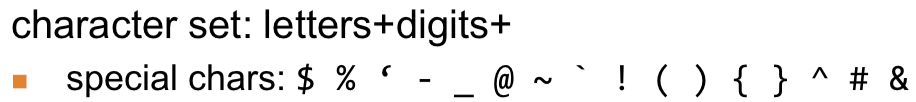
\includegraphics[width=0.75\linewidth]{images/char-set-msdos}\\
\emph{Type:} regular(ASCII, binary), directories, speical files(devices, symbolic links, named pipes). Distinguishing: extension(Win), magic number(Unix).
\emph{Protection:} Access control list, Permission bits(owner, group, other).\\
\emph{Structure:} array of bytes, fixed length record(instant access), variable length record(hard to locate).\\
\emph{Access method:} sequential access(rewound), random access(read, seek), direct access(on fixed length record, general random on record).

\subsection*{Directory}
Single-level, tree-structured (every node has only one parent), DAG (aliases, appear in multiple directories), general graph (achieved with symbolic link, infinite path possible -> maximum traversal limit in Unix).\\
\emph{Unix symbolic link:} Special link file contains path name. ln -s. Recursive. Win: shortcut does not re-expand further(not recursive).